\documentclass{UoYCSproject}
\addbibresource{REFERENCES.bib}

\usepackage{tikz}
\usetikzlibrary{automata, positioning, arrows}

\tikzset{
  ->, % makes the edges directed
  node distance=4cm, % specifies the minimum distance between two nodes. Change if necessary.
  every state/.style={thick, fill=gray!10}, % sets the properties for each ’state’ node
  initial text=$ $, % sets the text that appears on the start arrow
}

\newenvironment{monospace}{\ttfamily}{\par}

\BEng
\supervisor{Dr. Christopher Crispin-Bailey}

\begin{document}

\title{Generation of Hardware Accelerators for an FPGA System}
\author{Jay Valentine}

\maketitle

\begin{abstract}
\end{abstract}

\chapter{Introduction}

\section{Motivation}

With the breakdown of Dennard scaling and the observation of dark silicon in modern microprocessors,
we are rapidly approaching a utilization wall, meaning that not all transistors on a given chip can be utilized
simultaneously \cite{darksilicon}. This has severe consequences for the future of microprocessor architecture,
especially in domains where energy consumption is of great concern, such as the rapidly growing mobile application domain.

Because of this, research is turning towards novel architectures as a solution to this problem.
One such architecture is the \textit{coprocessor-dominated architecture} (\textit{CoDA}), in which one or more general-purpose
processing cores are coupled with a large number of specialised hardware accelerators, which are able to perform very specific
tasks with greater energy efficiency than a general-purpose core.

\section{Aims}

This work aims to show that such an architecture can be utilized in an embedded FPGA platform.
The use of an FPGA allows the accelerators to be designed specifically with the embedded application in mind.
The aim is to produce a tool that can generate hardware accelerators from an application written for the Xilinx MicroBlaze
soft processor \cite{microblaze}.

Because the accelerators are automatically generated by the tool, rather than designed by hand, the architecture
can be re-generated for each version of the application, or even across different applications, very easily.
The use of an FPGA allows the architecture to be very highly specialized, as the FPGA can be re-programmed for each architecture
version. In this sense, the architecture itself becomes an extension of the application software, rather than a static
platform as has traditionally been the case.

\chapter{Literature Review}

\section{Moore's Law and Dennard Scaling}

In 1965, Gordon Moore predicted that the number of transistors in an integrated circuit will double
approximately every two years  \cite{moore}. Similarly, Dennard scaling describes the way in which transistor power density
remains constant as the transistors themselves shrink in size \cite{dennard}. These phenomena combined allow for exponential
transistor-density increases, and this has been exploited to produce exponentially higher performance in
microprocessors year on year.

\begin{figure}[h]
\center{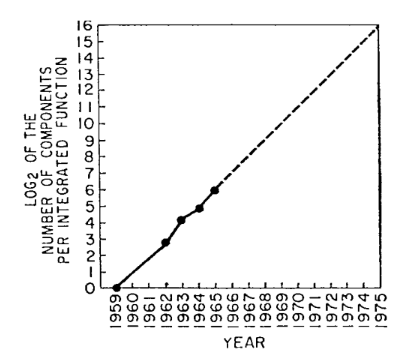
\includegraphics[width=\textwidth]
{figures/moore.png}}
\caption{Moore's 1965 prediction. \cite{moore}}
\end{figure}

However, in more recent times, a breakdown in this scaling has been observed. In the past, Dennard scaling has allowed
microprocessor manufacturers to offset the increased energy cost of faster transistor switching, resulting in higher
and higher clock speeds. However, more recently, microprocessor clock speeds have remained relatively static. This is
due to a breakdown in Dennard scaling for very small transistors, and has caused microprocessor manufacturers to instead
pursue increased performance by the use of multicore designs.

\begin{figure}[h]
\center{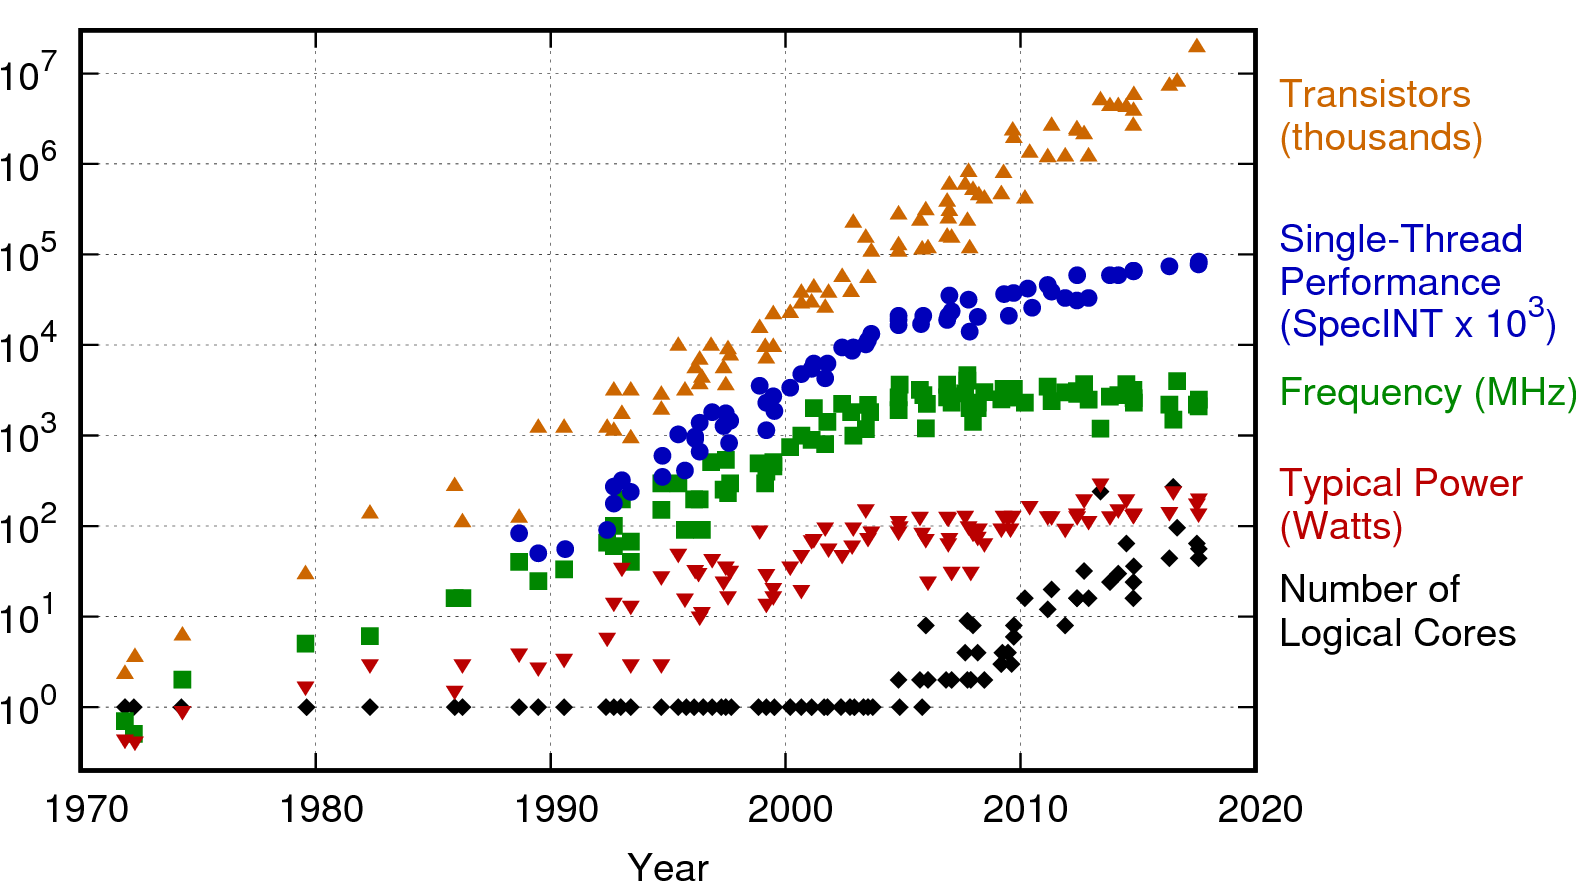
\includegraphics[width=\textwidth]
{figures/cpu-speed.png}}
\caption{Trends in microprocessors since 1970. \cite{karlrupp}}
\end{figure}

\section{Dark Silicon}

Dark silicon is a phenomenon which has been observed as transistor density in microprocessors has increased.
It occurs as transistor under-utilization leads to a gap between the speedup observed and that predicted by
extrapolating from historic performance gains.

In \cite{darksilicon}, it is predicted that with 22nm transistors, 21\% of the chip will be dark silicon,
with this rising to 50\% at 8nm. This prediction shows that dark silicon will become a serious limitation
as transistor density grows, especially in areas where energy efficiency is a primary concern.

Dark silicon also becomes a limiting factor with manycore devices. Even when energy consumption is not a
concern, the limited parallelism of most applications results in a dark silicon gap when running with
manycore devices. Again, \cite{darksilicon} shows that beyond a certain number of cores the speedup achieved
is negligible. This is another kind of dark silicon - the underutilization in this case is not a result of
energy concerns but is caused by the limited parallelism of the application being unable to exploit all of
the cores of a device.

There have been several broad responses to this phenomenon.
In \cite{four-horsemen}, Taylor gives two pessimistic predictions regarding the future of silicon
utilization. The first, the 'shrinking horseman', predicts that chips will begin to shrink as a result of
the utilization wall. This would lead to an increase in cost per mm\textsuperscript{2} of silicon, as
design costs, test costs, marketing costs, etc. Put simply, "exponentially smaller chips are not
exponentially smaller".

The second, perhaps slightly less pessimistic, prediction in Taylor's paper
is referred to as 'the dim horseman', and describes the under-clocking or infrequent use of
general-purpose silicon in order to meet power budgets. While a better alternative than the shrinking
of chips, this still causes issues as the chip is no longer operating at maximum capacity.
Taylor outlines several options for the use of this 'dim silicon'. The first, and perhaps most obvious,
is the use of homogenous architectures, but with some cores operating at a lower clock speed, or
even being turned off intermittently. However, there are other 'dim silicon' approaches that make better
use of the unutilized silicon area. One approach is to increase cache sizes, as cache memory is less
power-dense than a processing core would be. This has a secondary benefit as well, in that a larger
cache will reduce the number of cache misses, thereby decreasing the number of power-hungry off-chip
accesses.

Finally, Taylor also describes 'the specialized horseman'. This approach is to use the dark silicon area
not for general-purpose computing, but for a large number of specialized cores, which would be much
more energy efficient than a general-purpose core, allowing for increased energy efficiency at the
cost of silicon area.

\section{Heterogeneous Architectures}

One such 'specialized horseman' approach is the use of heterogeneous architectures.
These are computer architectures in which one or more general-purpose cores are coupled with special-purpose coprocessors,
also known as hardware accelerators. A hardware accelerator is a specialised hardware circuit intended to perform a
specific task more efficiently than a general-purpose processor. While historically hardware accelerators have been designed by
hand for a specific application (e.g. encryption), this is infeasible when considering architectures
with large numbers of accelerators. Thus an automated approach to generating hardware accelerators is required.

This is the approach taken in \cite{high-performance-microarchitecture}. Here Razdan and Smith propose a simple
hardware accelerator architecture which avoids the need for memory synchronization and reduces the overheads involved in
invoking a hardware accelerator. They describe a toolchain which is able to extract instruction streams to be 'outsourced' to an
accelerator core (called a \textit{programmable functional unit}, or \textit{PFU}) after code generation.

\begin{figure}[hbt]
\center{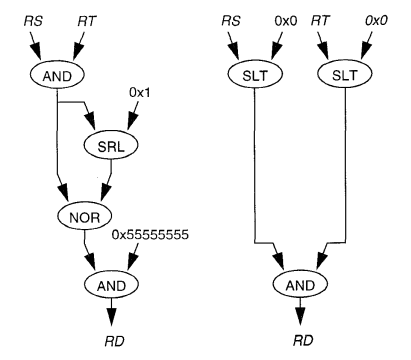
\includegraphics[width=0.75\textwidth]
{figures/pfu.png}}
\caption{Two PFU optimization examples. Both sequences of operations can be evaluated in a single cycle, while the same sequences in MIPS R2000 instructions would take multiple cycles. \cite{high-performance-microarchitecture}}
\end{figure}

The PFU model is a simplification from the general model of a hardware accelerator, which is as a multi-cycle state machine.
Instead each PFU has at most two input operands and at most one output operand. In addition, the PFU-logic instructions (MIPS
instructions that are candidates for translation into a PFU) cannot be memory-access or flow control instructions. This means
that each PFU has an identical interface, and can be executed in a single cycle. This allows PFUs to be executed with a single
instruction, \textit{expfu}, in a single cycle, maintaining the fixed-format and single-cycle instructions of the MIPS
processor's RISC instruction set.

\section{Conservation Cores}

While traditionally hardware accelerators have been used to speed up certain computations, they can also be used to achieve the
same computational performance as a general-purpose processor at a fraction of the energy cost, thus alleviating the dark silicon
problem.

\cite{c-cores} introduces \textit{conservation cores} (\textit{c-cores}), which are hardware accelerators
designed for this purpose. The paper outlines a method for generating c-cores for a given application.
The first step is to identify 'hot' and 'cold' portions of the application, using some form of profiling.
'Hot' code sections are those which are run frequently, and so are ideal candidates for c-cores. 'Cold' sections
are run infrequently, and so are not ideal candidates, as the overhead involved in using a c-core would
not be offset by the computation avoided by its use.

Once 'hot' portions are identified, a c-core can be synthesised for it. While previous hardware accelerators
might have been hand-designed, such an approach is not viable if large numbers of c-cores are to be used, and so
the paper outlines a method for automating the synthesis of these cores. A control-flow graph can be extracted
from the code, and from this a state machine model can be constructed to perform the functionality represented
in the code. This state machine can then be implemented in a language such as VHDL or Verilog, and from this a circuit
can be synthesised.

\begin{figure}[h]
\center{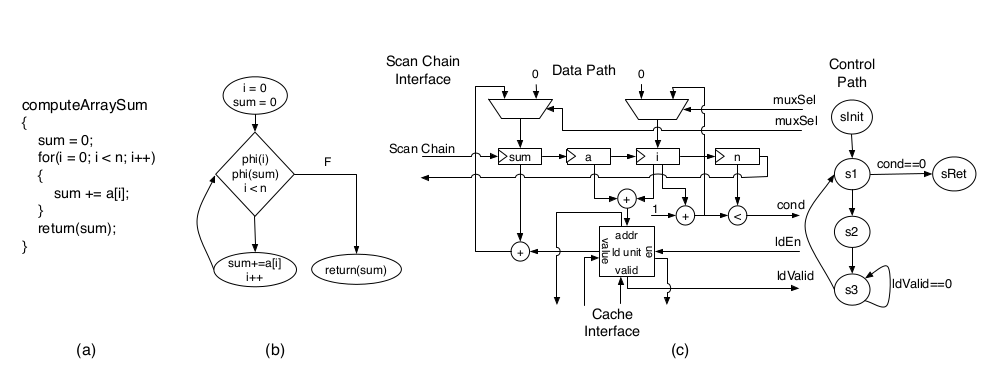
\includegraphics[width=\textwidth]
{figures/c-cores.png}}
\caption{Conservation core example. \cite{c-cores}}
\end{figure}

One of the main issues with these c-cores is that memory synchronization restricts ILP (instruction-level parallelism)
and requires large numbers of pipeline registers (as each memory access marks a state-boundary). \cite{eco-cores} attempts
to alleviate this issue by introducing \textit{selective de-pipelining} (SDP), in which memory accesses occur in 'fast states'
while the rest of the processing done by the c-core proceeds as before, in 'slow states'.

Signals can safely propogate through the entire block without the need for latching on fast-state boundaries,
while values loaded from memory are latched on fast-state boundaries as soon as they are available.
An example of this process is shown in figure 2.4.

\begin{figure}[h]
\center{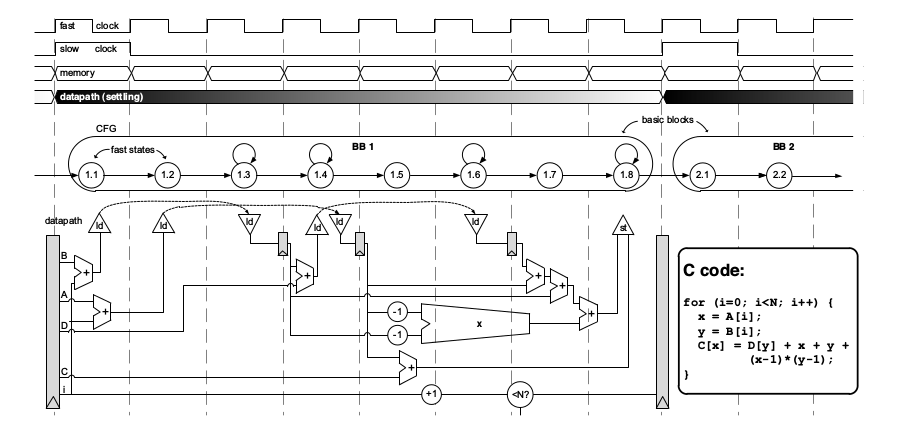
\includegraphics[width=\textwidth]
{figures/sdp.png}}
\caption{Selective de-pipelining example. \cite{eco-cores}}
\end{figure}

The GreenDroid project \cite{greendroid} takes the ideas of both \cite{c-cores} and \cite{eco-cores} and attempts
to apply them to the Android operating system and software stack. Mobile phone processors have vastly lower power budgets than
traditional desktop processors, both to achieve long battery life and to reduce generated heat. Profiling of the Android
software was used to identify the best portions of code to be converted into c-cores. As a result,
c-cores account for over 90\% of execution time, and if clock-gated when not in use (leaving them idle and consuming
very little power), this leads to a significant reduction in energy consumption.

A similar approach is taken by Arnone in \cite{arnone-thesis}. Here, Arnone outlines a method of
generating accelerator cores for a stack architecture, resulting in both timing
and power improvements. Two architectures for generated cores are described: composite and wave-core.
Composite cores are simple state machines with instructions mapped to states. Composite cores attempt to
optimise for logic area by reusing existing logic between states. Conversely, the wave-core
architecture avoids the reuse of logic between states, reducing power density at the cost of increased
logic area (due to potentially duplicated functionality). In both cases the resulting accelerator core is
more energy-efficient than the general-purpose processor is at the same task.

Here each core is a finite state machine generated from a basic block in the stack architecure's
assembly code. States are divided between computation states and memory-access states. Each computation state
is formed of a series of HDL (VHDL is used, but this could just as easily be Verilog) statements which are direct
translations of instructions in the stack architecture's instruction set. Between each computation state are one
or more states in which memory is being accessed, to either load or store data. Outputs from each state are latched
in registers so that they are available for the next state to operate on. Because each computation state is a simple
data-flow system with no need for synchronization, they can be completed within a single cycle.

These cores differ from conservation cores in that there is no control flow - while c-cores can encode loops, Arnone's
work focuses solely on basic blocks. This means that less use can be made of the cores (as the main processor must still
perform flow control), but also that the implementation of state machines is less complex - they are linear.

\chapter{Methodology and Design}

\section{System Architecture}

MicroBlaze \cite{microblaze} is a 32-bit RISC architecture. It is highly configurable, as certain features (e.g. FPU, multiplier, barrel shifter)
can be disabled if not required. This allows the architecture to be as minimal as is required by the application.

The system used in this project consists of one MicroBlaze core, connected to local instruction and data block RAM (BRAM)
via the local memory bus (LMB). The processor's AXI bus is used to connect to one or more hardware accelerator cores.
These hardware accelerator cores are then connected to the BRAM via a standard Xilinx BRAM interface.

\begin{figure}[h]
\center{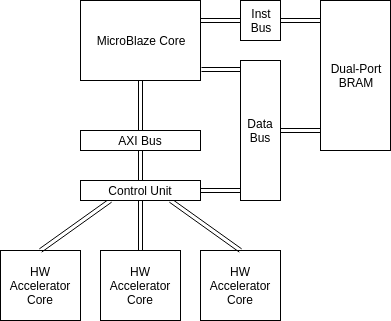
\includegraphics[width=\textwidth]
{figures/architecture.png}}
\caption{System architecture.}
\label{fig:systemArchitecture}
\end{figure}

The LMB is intended for connecting the MicroBlaze core to on-chip BRAM, for use as a local cache memory, with instructions
and data being stored in off-chip flash or DRAM. The system topology described above allows for a tiled architecture,
with each block containing a MicroBlaze core and several hardware accelerators. Each tile would have its own local memory,
with these memories being connected in turn (via some kind of cache interface) to the system-wide main memory. However,
this is beyond the scope of this project, which focuses on a single MicroBlaze core with associated accelerators,
and a single BRAM, with no main flash or DRAM.

\section{Hardware Accelerator Model}

\section{Code Analysis}

In order to identify the best candidates for extraction into hardware accelerators, some analysis needs to be performed.
The first step in this analysis is to break the instruction stream up into basic blocks. A basic block is a linear portion of
code, bounded at both ends by flow control instructions (e.g. branch or call instructions). These blocks can then be linked
together into a data-flow graph, in which all nodes are basic blocks, and all edges links between those blocks.

\subsection{Inputs and Outputs}

From this representation, some information about the individual blocks can be extracted. It is possible to know what the inputs
and outputs from a block are in isolation (with an input being any register that is read before being written to in the block,
and an output being any register written to at any point in the block). However, this leads to very conservative results, as
highlighted by figure ~\ref{fig:analysisNaiveApproach}. In the example, \texttt{r6} is used as a temporary register, and
according to the MicroBlaze ABI \cite{microblaze-ref} is discarded on returning from the function. If we take the naive approach
to identifying a block's outputs, we ignore this fact and assume that because \texttt{r6} is written to, it must be an output of
the block. In a real block, there may be many more temporary registers used, resulting in the analysis reporting a large number
of 'false outputs'.

\begin{figure}[h]
  \begin{center}
    \begin{minipage}{0.5\linewidth}
      \begin{monospace}
      lwi r3,r5,0

mul r6,r3,r3

addik r3,r6,20

rtsd r15, 8

inputs: r5

outputs: r3, r6

      \end{monospace}
    \end{minipage}
  \end{center}

  \caption{A naive approach to basic block analysis.}
  \label{fig:analysisNaiveApproach}
\end{figure}

In order to solve this problem, the analysis needs to take into account both how the registers are used (as defined by the
ABI) and the context in which the block exists (i.e. what blocks come before and after it).

\subsection{Input/Output Overheads}

For every input or output register to a block which is to be converted to an accelerator, the data contained within that register
must be transferred between the processor and the hardware accelerator core. The cycles of overhead for a particular core are
given by:

\begin{center}
\[ (\#inputs \times cycles_w) + (\#outputs \times cycles_r) \]
\end{center}

Where \(cycles_w\) and \(cycles_r\) are the number of cycles taken for a read from or write to the hardware accelerator,
respectively.

This means that as the number of inputs or outputs of a block increase, the benefits of converting that block to a hardware
accelerator will diminish.

\subsection{Memory-Access Density}

The simple hardware accelerator model being used is that of a state machine which alternates between 'wait' states,
in which the hardware accelerator is waiting on memory for a read or write operation, and 'computation' states,
in which the hardware accelerator is calculating some values based off its internal registers. While computation states
can be completed in a single clock cycle, the hardware accelerator may spend several cycles in a wait state, depending
on the memory latency. Even in the best case, the accelerator will spend at least a single cycle in each wait state.

Because of this, if the translated block contains a large amount of memory-access instructions, and a small amount of computation,
the accelerator may not provide much of an increase in execution speed over the general purpose processor. Consider the block
shown in figure ~\ref{fig:highMemoryDensity}: the generated accelerator will alternate between wait and computation states,
with each computation state containing at most a single instruction. The accelerator will consume the same number of cycles
executing this operation as the general-purpose processor.

\begin{figure}[h]
  \begin{center}
    \begin{minipage}{0.5\linewidth}
      \begin{monospace}
      lwi r4,r5,0

addk r3, r3, r4

lwi r4, r5, 4

addk r3, r3, r4

lwi r4, r5, 8

addk r3, r3, r4

lwi r4, r5, 12

addk r3, r3, r4

      \end{monospace}
    \end{minipage}
  \end{center}

  \caption{A block with high memory-access density.}
  \label{fig:highMemoryDensity}
\end{figure}

Some of these issues can be overcome by compiler optimisation. A compiler could ensure that all the memory access in the example
is done 'up front', resulting in 3 wait states and 1 computation state. However, if there are dependencies between
the memory accesses, such an optimization may not be possible.

\section{Translation into State Machines}

\begin{figure}[ht]
  \centering
  \input{figures/autogen/statemachine.tex}
  \caption{An example hardware accelerator model.}
  \label{fig:exampleStateMachine}
\end{figure}

\printbibliography

\end{document}